\documentclass[a4paper,10pt]{article}

\usepackage{amsmath}
\usepackage{amsfonts}
\usepackage{amssymb}
\usepackage{amsthm}
\usepackage{fourier}
\usepackage{multirow}
\usepackage{graphicx}
\usepackage{booktabs}
\usepackage{xcolor}
\usepackage{tikz}
\usepackage[a4paper, margin=.5in]{geometry}
\usepackage{hyperref}

\usetikzlibrary{arrows.meta, positioning}
\newtheorem{assumption}{Assumption}
\newtheorem{lemma}{Lemma}
\newtheorem{remark}{Remark}

\newcommand{\todo}[1]{\textcolor{red}{#1}}

\title{}
\date{}
\author{}

\begin{document}
\maketitle

% =======================================================================================
\section{Introduction}
% =======================================================================================

Advanced cancer is harder to treat than early-stage cancer. As patients move through successive lines of therapy, they build up side effects, sometimes lasting organ damage, and their treatment options become narrower. Metastatic cancer, where tumor cells have spread through the body, is one of the most difficult of these stages. Relapse is frequent, mortality is high, and every decision must weigh the risk of the disease progressing against the growing burden of treatment. This complexity also makes new therapies hard to test: clinical trials need strict eligibility criteria to control patient heterogeneity, progression is hard to detect early, and the competing risks of toxicity and disease activity make trials more likely to fail.

Metastatic breast cancer (mBC) is one of the most studied examples of this challenge, and new therapies are being developed quickly. Breast cancer is classified by its hormone receptor profile into three main subtypes: HR+/HER2-, HER2+, and triple-negative (TN). These subtypes differ in biology, prognosis, and available treatments. The triple-negative subtype is the most aggressive, while HR+/HER2-, the most frequent, is the best characterized. Population-level figures, however, hide large differences between individual patients. These differences come from tumor biology, patient characteristics, and the pressure of earlier treatments. As a result, predicting how a given patient will do, and choosing the best treatment for that patient, remains a hard clinical problem.

\paragraph{How treatment is organized in mBC.}
Treatment for mBC is organized into successive lines of therapy. A line ends at progression, that is, when new metastases appear or existing ones grow. Within each line, the choice of treatment follows subtype-specific guidelines, which are built for populations rather than for individual patients. The further a patient goes through the lines, the less these guidelines fit: the patient's profile moves away from the population the guidelines were built on, and the set of reasonable options becomes harder to navigate. Testing every possible sequence of treatments would require a very large number of clinical trials. Real-world medical records offer a complementary source of evidence. They follow patients through their whole treatment history, as it happens in routine care, and at a scale no trial can reach.

\paragraph{Why causal inference is needed.}
Real-world data cannot, however, be used naively to compare treatments. Treatment is not assigned at random: it depends on the patient. Sicker patients, or patients with more aggressive disease, may be more or less likely to receive a given treatment. Comparing outcomes across treatment groups, for instance with a Cox model fitted to each group, then mixes the effect of the treatment with the differences between the patients who received it. This is called confounding. Randomized trials remove confounding by design. With observational data, causal inference gives a framework to recover treatment effects under explicit assumptions. Target trial emulation applies this framework by first describing the trial one would like to run, and then using the observational data to imitate it as closely as possible \todo{[Hern\'an and Robins, 2016]}.

\paragraph{Survival analysis as the outcome framework.}
A natural way to compare treatments is survival analysis, which models the time from a starting point to an event such as death or progression. The Cox proportional hazards model is the classical reference. It is easy to interpret, but it assumes that the hazard ratio between groups stays constant over time. In the metastatic setting, where each patient's history is a sequence of treatments and progressions, static models also struggle to use information that changes over time. Neural network survival models relax these limits and have outperformed classical models in several settings. Placing survival analysis inside a causal framework takes one more step: it moves from ``which patients tend to live longer'' to ``how long would this patient live under this treatment rather than another''.

\paragraph{Contributions.}
In this work we build a treatment recommendation system for mBC from real-world treatment sequences. Our contributions are threefold:
\begin{itemize}
    \item[i.] A \emph{sequential causal survival model} that reads the full treatment history of a patient and predicts, for each candidate treatment, the overall survival curve from the start of the current line.
    \item[ii.] A \emph{recommendation procedure} that only gives advice where the data can support it. Treatments are filtered by sample size, by how well-defined they are, by available follow-up, and by a patient-specific positivity check. When no treatment passes, the system abstains. The procedure also measures its own uncertainty with an ensemble of models trained from different random initializations: when the treatments cannot be separated, it returns the short list of equivalent options instead of a single choice.
    \item[iii.] A \emph{data analysis} of the ESME HR+/HER2- cohort that explains these design choices: how treatments repeat along sequences, how calendar time changes both practice and outcomes, and how selection shapes later-line populations.
\end{itemize}

The paper follows this order. Section~\ref{sec:formulation} defines the problem, the causal structure, and the quantity we want to estimate. Section~\ref{sec:data} describes the cohort and the analyses that shape our design. Section~\ref{sec:model} presents the model, and Section~\ref{sec:recommendation} the recommendation procedure. Sections~\ref{sec:factual-validation} and~\ref{sec:counterfactual} evaluate the model, and Section~\ref{sec:discussion} discusses limitations and future work.

% =======================================================================================
\section{Problem Formulation and Causal Structure}
\label{sec:formulation}
% =======================================================================================

To compare treatments for a patient, we first need to state precisely what a patient trajectory is, how treatment decisions are made, and which quantity we want to estimate.

\subsection{Patient Representation}

Each patient is described by three sequences: $X_{1:L}$ the patient state, $A_{1:L}$ the treatments, and $Y_{1:L} := (P, O)_{1:L}$ the survival outcomes. At line $k$, $X_k$ is the patient's clinical state at the start of the line, $A_k$ the treatment given during the line, and $P_k$ and $O_k$ the progression-free survival and overall survival measured from the start of the line. In our data $L \leq 4$.

\subsection{Treatment Line Definition}

The first line starts when the patient begins treatment for metastatic disease. A line ends at progression, defined as the appearance of new metastases or the growth of existing ones. The next line starts when the next treatment begins. The time between the end of one line and the start of the next is called the \textit{buffer time}, denoted $d_k$.

\subsection{Causal Structure}

In observational data the treatment $A_k$ is not random. It depends on the patient's state $X_k$ and on what happened before. We write
\begin{equation}
    H_k^- := (X_{1:k-1},\, A_{1:k-1},\, P_{1:k-1})
\end{equation}
for the history before line $k$, and
\begin{equation}
    H_k := H_k^- \cup \{X_k\} = (X_{1:k},\, A_{1:k-1},\, P_{1:k-1})
\end{equation}
for everything the physician knows when choosing the treatment of line $k$. Because the choice depends on $H_k$, a model that simply links treatments to outcomes learns how physicians select patients, not what treatments do.

We therefore use a sequential causal structure that follows the clinical decision process. The joint distribution of a trajectory factorizes as
\begin{equation}
    P(X_{1:L}, A_{1:L}, P_{1:L}, O_{1:L})
    = \prod_{k=1}^{L}
    \underbrace{P(X_k \mid H_k^-)}_{\text{state transition}} \;
    \underbrace{P(A_k \mid H_k)}_{\text{treatment assignment}} \;
    \underbrace{P(P_k \mid H_k, A_k)}_{\text{progression-free survival}} \;
    \underbrace{P(O_k \mid H_k, A_k)}_{\text{overall survival}}
    \label{eq:factorization}
\end{equation}
with the convention $X_0 = A_0 = P_0 = \emptyset$. The factors of line $k$ are only defined for patients alive at the start of that line; a patient who dies during line $k$ contributes nothing beyond it.

Progression $P_k$ plays two roles in this structure. It is an outcome of line $k$, and it also shapes the next state $X_{k+1}$, since progression is the event that starts the next line and redefines the disease status. This is exactly why a static causal adjustment is not enough and a sequential view is needed.

\begin{figure}[h]
\centering
\scalebox{0.7}{
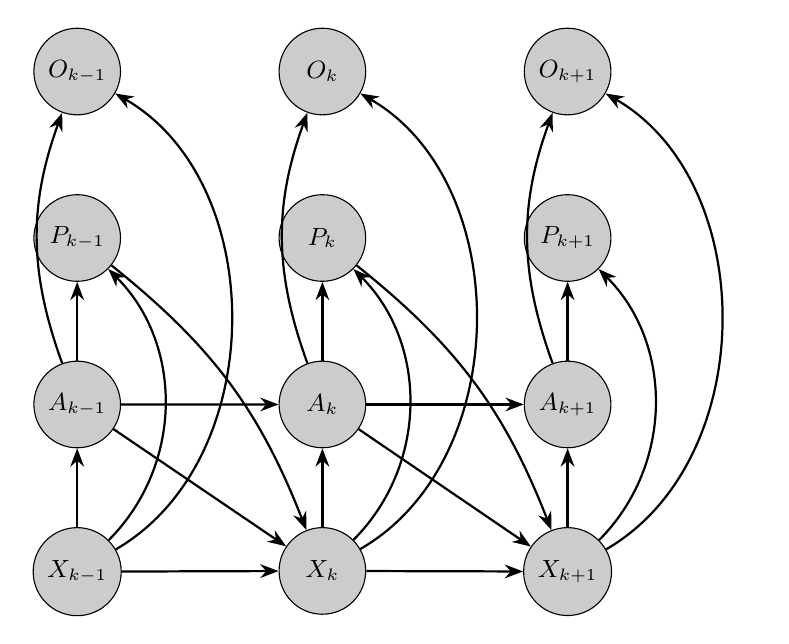
\begin{tikzpicture}[
    node distance=1.0cm and 2cm,
    arr/.style={-{Stealth}, thick},
    every node/.style={circle, draw, fill=gray!40, minimum size=1.1cm, font=\small},
]

    \node (O1) {$O_{k-1}$};
    \node[right=of O1] (O2) {$O_{k}$};
    \node[right=of O2] (O3) {$O_{k+1}$};

    \node[below=of O1] (P1) {$P_{k-1}$};
    \node[below=of O2] (P2) {$P_{k}$};
    \node[below=of O3] (P3) {$P_{k+1}$};

    \node[below=of P1] (A1) {$A_{k-1}$};
    \node[below=of P2] (A2) {$A_{k}$};
    \node[below=of P3] (A3) {$A_{k+1}$};

    \node[below=of A1] (X1) {$X_{k-1}$};
    \node[below=of A2] (X2) {$X_{k}$};
    \node[below=of A3] (X3) {$X_{k+1}$};

    \draw[arr] (X1) -- (A1);
    \draw[arr] (A1) -- (P1);
    \draw[arr] (A1) to[bend left=20] (O1);
    \draw[arr] (X1) to[bend right=45] (P1);
    \draw[arr] (X1) to[bend right=60] (O1);

    \draw[arr] (X2) -- (A2);
    \draw[arr] (A2) -- (P2);
    \draw[arr] (A2) to[bend left=20] (O2);
    \draw[arr] (X2) to[bend right=45] (P2);
    \draw[arr] (X2) to[bend right=60] (O2);

    \draw[arr] (X3) -- (A3);
    \draw[arr] (A3) -- (P3);
    \draw[arr] (A3) to[bend left=20] (O3);
    \draw[arr] (X3) to[bend right=45] (P3);
    \draw[arr] (X3) to[bend right=60] (O3);

    \draw[arr] (X1) -- (X2);
    \draw[arr] (X2) -- (X3);

    \draw[arr] (A1) -- (A2);
    \draw[arr] (A2) -- (A3);

    \draw[arr] (A1) -- (X2);
    \draw[arr] (A2) -- (X3);

    \draw[arr] (P1) to[bend left=15] (X2);
    \draw[arr] (P2) to[bend left=15] (X3);

\end{tikzpicture}
}
\caption{Sequential causal structure over treatment lines. $X_k$ is the patient state, $A_k$ the treatment, $P_k$ the progression-free survival, and $O_k$ the overall survival at line $k$. $O_k$ is a terminal node; $P_k$ feeds into the next state because progression starts the next treatment line.}
\label{fig:dag}
\end{figure}

Figure~\ref{fig:dag} shows this structure. At line $k$, the physician chooses $A_k$ based on the patient state $X_k$ and on the previous treatment $A_{k-1}$. \todo{This reflects the clinical practice of following treatment sequences and avoiding regimens that already failed; Section~\ref{sec:data} shows that categories are nonetheless often repeated.} Both $X_k$ and $A_k$ affect the two outcomes $P_k$ and $O_k$. Overall survival $O_k$ is a terminal node: death ends the trajectory, so $O_k$ has no outgoing edge. Progression $P_k$, on the other hand, points to $X_{k+1}$. The transition $X_k \rightarrow X_{k+1}$ also depends on $A_k$, which captures the direct effect of treatment on how the disease evolves.

\subsection{Causal Estimand}
\label{sec:estimand}

We can now state the quantity we want to estimate. At the start of line $k$, the physician chooses among treatments $a \in \mathcal{A}$. The question is: what would this patient's survival be if treatment $a$ were given? With potential outcomes, let $O_k(a)$ be the overall survival at line $k$ under treatment $a$, and $P_k(a)$ the progression-free survival. Both exist for every $a$, whatever treatment was actually given.

Our estimand is the survival curve under treatment $a$, given the history:
\begin{equation}
    S_a(t \mid H_k) := \mathbb{P}\big(O_k(a) > t \mid H_k\big), \qquad t \in \{1, \ldots, T\},\; a \in \mathcal{A}.
    \label{eq:estimand}
\end{equation}
To compare treatments with a single number, we use the restricted mean survival time (RMST) up to a horizon $\tau$:
\begin{equation}
    \text{RMST}_a(\tau \mid H_k) = \int_{0}^{\tau} S_a(t \mid H_k)\, dt,
\end{equation}
which is the expected number of months lived within the first $\tau$ months of the line. RMST does not rely on proportional hazards, and it is directly readable by clinicians \todo{[Royston and Parmar, 2013]}.

\paragraph{What the intervention is.}
Equation~\eqref{eq:estimand} describes a \emph{single-line intervention}. We set $A_k = a$ and let the following treatments $A_{k+1:L}$ be chosen as they normally are in practice. The effect we estimate is therefore a \emph{total} effect. It includes the direct effect of treatment $a$, and an indirect effect that goes through the later treatments that choosing $a$ tends to lead to. We do not try to separate the two. Isolating the direct effect would require the identifying assumptions to hold at every future line, a model of how the patient state evolves under each treatment, and a simulator that chains these models forward. Including the indirect path is not a source of bias: future treatments come after $A_k$ in the graph of Figure~\ref{fig:dag}, so they are consequences of $A_k$, not common causes of $A_k$ and $O_k$.

This total effect is also the quantity that matches the clinical decision. At the start of line $k$, the physician only commits to $A_k$. Later decisions will be made later, by the same care system that produced the data, based on how the patient evolves. The useful question is therefore not ``what does $a$ do in isolation from all later care?'', which no real intervention can produce, but ``what happens if we choose $a$ now, knowing that later care will unfold as usual for patients like this one?''. Our estimand answers this second question. Its validity depends on later care in deployment staying close to the care observed in the training data. This is one reason we validate on a temporal split (Section~\ref{sec:data}).

\paragraph{Single-line recommendation, not an optimal sequence.}
Our framework recommends one line at a time. It does not claim to find the best full sequence of treatments. Choosing the best treatment at each line separately does not, in general, give the best sequence: the choice at line $k$ changes the patient's future state, and hence how well later options will work. A treatment that looks worse at line $k$ could lead to a state in which later lines work much better, and the reverse is also possible. Optimizing whole sequences is a dynamic treatment regime problem. It can be addressed with backward induction (Q-learning, G-estimation) or off-policy reinforcement learning, but these methods need stronger assumptions and a model of state transitions under each treatment. We come back to this in Section~\ref{sec:discussion}.

\subsection{Identifiability}
\label{sec:identifiability}

To estimate $S_a(t \mid H_k)$ from observational data, it must be possible to write it in terms of the observed data distribution. This relies on three standard assumptions. Our data analysis (Section~\ref{sec:data}) shows that the first two do not hold everywhere in the raw data, and we explain how the cohort and the recommendation procedure are built to respect them.

\begin{assumption}[Consistency]
The observed outcome of a patient who received treatment $A_k = a$ equals the potential outcome under $a$:
\begin{equation}
    A_k = a \implies O_k = O_k(a), \quad P_k = P_k(a).
\end{equation}
\end{assumption}
Consistency requires each treatment to be one well-defined intervention. This holds reasonably well for most treatment categories, but not all. The category \textsc{other} groups 736 distinct drug combinations, and its most common combination covers only 16\% of its records. The category \textsc{et+tt} groups 344 combinations. ``Give \textsc{other}'' is therefore not a single action, and its estimated effect would average over a mix of regimens that may change at deployment \todo{[VanderWeele and Hern\'an, 2013]}. \textsc{no treatment} appears 207 times at line 1 and almost never afterwards, which points to a coding artifact rather than a therapeutic choice. We keep the records of these three categories in the patient histories, but we never recommend them (Section~\ref{sec:recommendation}).

\begin{assumption}[Positivity]
For every line $k$ and every treatment $a \in \mathcal{A}$, every possible history has a non-zero chance of receiving $a$:
\begin{equation}
    P(H_k) > 0 \implies P(A_k = a \mid H_k) > 0.
\end{equation}
\end{assumption}
Positivity ensures that each treatment has been observed in patients similar to the one we want to advise. In our data it is violated in two different ways. The first is \emph{availability}: some treatments did not exist for part of the study period. CDK4/6 inhibitors were approved in Europe at the end of 2016, so a patient treated in 2010 had exactly zero chance of receiving them. No adjustment can create evidence for such a patient. The second is \emph{sparse support}: some treatments are rarely given at a given line, or rarely given to patients with a given profile. These two problems need different answers. We handle availability by restricting the cohort to a period in which the set of available treatments is stable, and by adding calendar time as a covariate inside that period, where it becomes an ordinary confounder (Section~\ref{sec:data}). We handle sparse support with per-line and per-patient eligibility filters (Section~\ref{sec:recommendation}) \todo{[Petersen et al., 2012]}.

\begin{assumption}[Sequential Ignorability]
Given the observed history, the treatment at each line is independent of the potential outcomes:
\begin{equation}
    A_k \perp\!\!\!\perp \{O_k(a), P_k(a)\}_{a \in \mathcal{A}} \mid H_k.
\end{equation}
\end{assumption}
This is the key assumption. It states that all factors that influence both the treatment choice and the outcome are recorded in the history $H_k$. It cannot be tested from observational data. Restricting the cohort and filtering treatments do not help here: they deal with positivity and consistency, not with unmeasured confounders such as patient preference, frailty, or the physician's overall impression. Our data analysis also shows that age is not available and that performance status is partly imputed (Section~\ref{sec:data}). We therefore treat ignorability as the main open assumption of this work. \todo{A sensitivity analysis for unmeasured confounding (e.g.\ E-values, [VanderWeele and Ding, 2017]) will be added.}

\begin{lemma}[Identifiability]
\label{lem:identifiability}
Under Assumptions 1--3, and assuming that censoring is independent of survival given $(H_k, A_k)$, for every $a \in \mathcal{A}$ and every history $H_k$ with $P(H_k) > 0$,
\begin{equation}
    S_a(t \mid H_k) = \mathbb{P}\big(O_k > t \mid H_k, A_k = a\big).
\end{equation}
\end{lemma}
In words, the counterfactual survival curve equals the observed survival curve of patients with the same history who received $a$. The proof is given in Appendix~\ref{app:identifiability}. This result is what the model estimates: one survival curve per treatment, conditional on the history.

% =======================================================================================
\section{Data and Cohort Analysis}
\label{sec:data}
% =======================================================================================

The formulation above rests on assumptions about the data. Before building the model, we studied the cohort to check these assumptions and to decide how the cohort, the covariates, and the validation should be defined. This section presents the data and the four findings that shaped our design.

\subsection{Data Source and Record Construction}

We use the HR+/HER2- population of the Epidemiological Strategy and Medical Economics (ESME) metastatic breast cancer cohort, a French real-world database collected in \todo{18} comprehensive cancer centers. Over the first four lines, the full data contain 19,865 patients and 63,317 line records, with treatments grouped into 11 categories.

For each patient and each line $k$ at which the patient is alive, we build one record. It contains the medical history summarized up to the progression of line $k-1$ (or up to metastatic diagnosis at $k=1$), together with the treatment $A_k$ given at line $k$. This record is the observed version of the pair $(H_k, A_k)$ of Section~\ref{sec:formulation}. The outcomes are the progression-free survival $P_k$, from the first day of line $k$ to the next progression, and the overall survival $O_k$, from the first day of line $k$ to death or censoring. Patients who died during an earlier line contribute no later records.

Two consequences follow. First, the prediction target at line $k$ is survival from the start of line $k$, for patients alive at that point. Second, the history includes all previous treatments and progressions, so the model can use the full sequence of past decisions and responses.

\subsection{Finding 1: Treatment Categories Are Often Repeated}

We first looked at how treatments follow each other. Among the 7,131 patients with four lines, 75\% receive the same treatment category more than once within these four lines (Figure~\ref{fig:repeats}). Repeats are not only continuations from one line to the next: 22\% of patients come back to a category after switching to a different one. All 15 possible repeat patterns over four lines occur in the data.

This means that the treatment given at a line is strongly tied to the treatments given before, and not only to the previous one. A model that looks at each line on its own would miss this information. This motivates a sequential encoder that reads the full treatment history (Section~\ref{sec:encoder}).

\begin{figure}[h]
\centering
\includegraphics[width=.85\linewidth]{figs/treatment_category_repeats.png}
\caption{Repetition of treatment categories over the first four lines (patients with four lines). Left: patients by kind of repetition. Middle: repetitions per category, split into consecutive repeats and returns after a switch. Right: all 15 repeat patterns.}
\label{fig:repeats}
\end{figure}

\subsection{Finding 2: Calendar Time Changes Both Practice and Outcomes}

The treatment mix changed strongly over the study period. Endocrine therapy combined with CDK4/6 inhibitors was absent before 2014 and reached 66\% of first-line treatments in 2022. Chemotherapy combined with anti-angiogenic agents went the other way, from 12--16\% of first-line treatments to about 0.3\%. Calendar time also drives follow-up: death is observed for 94\% of patients who started in 2008, but for only 21\% of those who started in 2022, simply because recent patients have been followed for less time.

Calendar time was not among the model covariates, and ignoring it gives a misleading picture of positivity. With a propensity model that ignores calendar time, only 0.4\% of patients have a probability below 0.01 of receiving CDK4/6 inhibitors. Once the start year is added, this share rises to 36.5\%. The apparent overlap came from pooling periods in which the treatment did and did not exist.

Within each treatment category, crude first-line survival is essentially flat over 15 years (Figure~\ref{fig:km-year}). The differences between categories reflect which patients receive each treatment, not treatment effects. To test whether standard adjustment could make categories comparable over the whole period, we reweighted each group with inverse probability of treatment weights (80 covariates including calendar year) and inverse probability of censoring weights. The adjustment works for the categories used throughout the period: after weighting, the largest standardized mean difference is at most 0.07 for endocrine therapy alone, polychemotherapy, monochemotherapy, and \textsc{other}. It fails for the categories tied to a period: the remaining imbalance is 0.42 for CDK4/6 inhibitors and 0.38 for anti-angiogenic combinations, and it sits on the year indicators (Figure~\ref{fig:adjustment}). No weighting can make a 2010 patient a plausible recipient of a 2018 drug. This is the availability problem of Section~\ref{sec:identifiability}, visible directly in the data.

\begin{figure}[h]
\centering
\includegraphics[width=.8\linewidth]{figs/km_line1_24mo_trend.png}
\caption{Crude 24-month overall survival from the start of line 1, by calendar year and treatment category. Survival is flat within categories; the gaps between categories reflect patient mix, not treatment effects.}
\label{fig:km-year}
\end{figure}

\begin{figure}[h]
\centering
\includegraphics[width=.85\linewidth]{figs/km_line1_adjustment_diagnostics.png}
\caption{Diagnostics of the inverse probability weighting at line 1: covariate balance before and after weighting, effective sample size, and overlap over calendar time. Balance fails for the categories that were only available during part of the period.}
\label{fig:adjustment}
\end{figure}

\paragraph{Design decision.} We restrict the cohort to patients whose \emph{first} line starts in 2018 or later. By 2018, CDK4/6 inhibitors were already in routine use and anti-angiogenic combinations had disappeared, so the set of available treatments is stable over the window. Selecting on the first line, rather than on each line separately, keeps every patient's trajectory complete. Inside the window, calendar time only reflects gradual changes in practice, which is ordinary confounding. We therefore add the time since the start of the window as a covariate. Within the window, a propensity model using calendar time alone predicts treatment no better than chance (AUC 0.50--0.54 at every line).

\subsection{Finding 3: Later-Line Improvements Are Partly Case Mix}

At line 1, survival did not improve materially over calendar time. Lines 2 to 4 seem to tell a different story: crude 12-month overall survival rose by 4.3, 10.9, and 11.9 points between 2008--2011 and 2020--2024. However, the patients reaching these lines also changed. For example, the share of line-4 patients previously treated with CDK4/6 inhibitors went from zero before 2016 to about 70\% by 2020--2024. When we hold the previous treatments fixed by direct standardization, the gains shrink to 1.1, 5.1, and 5.5 points (Figure~\ref{fig:later-lines}). Moreover, what remains happened between 2008--2011 and 2012--2015 and stayed flat afterwards, including after CDK4/6 inhibitors arrived.

Selection adds to this effect. Reaching line $k$ means having progressed and survived through all earlier lines. After CDK4/6 inhibitors arrived, fewer patients reached later lines: within four years of starting line 1, the share reaching line 2 fell from about 70\% to 59\%, and the share reaching line 4 from about 33\% to 26\%. Those who did reach them took about as long as before (median 11.9 to 13.1 months to line 2, 27.8 to 28.0 months to line 4). Later-line populations therefore became smaller and more selected.

\begin{figure}[h]
\centering
\includegraphics[width=.7\linewidth]{figs/km_later_lines_trend.png}
\caption{12-month overall survival at lines 2--4 by calendar period. Top: trends within groups of patients with the same previous treatments. Bottom: crude versus history-standardized survival. The gap between the two is the part of the apparent improvement explained by who reaches the line.}
\label{fig:later-lines}
\end{figure}

\paragraph{Design decision.} Survival at a later line can only be interpreted once the treatment history is taken into account. This supports conditioning on the full history $H_k$, as in Section~\ref{sec:formulation}, rather than on the current state alone. It also explains why a model trained on all lines together must deal with populations that differ from line to line (Section~\ref{sec:calibration}).

\subsection{Finding 4: Imputed Covariates Can Create False Trends}

Performance status (ECOG/WHO, from 0 = fully active to 4 = completely disabled) is available in two forms: dated raw measurements, and an imputed value with no missing data, which is the one used by the model. The raw measurements show a modest worsening over time: between 2008--2012 and 2018--2022, the share of patients with status 0 fell from 42.0\% to 37.1\%, and the share with status 2 or more rose from 18.9\% to 22.9\%. The imputed values show the opposite trend for status 0, which rises from 21.9\% to 28.5\%.

This reversal comes from missing data, not from the patients. Only 31\% of patients starting line 1 in 2008 have a measurement within 90 days of the line start, compared with 80\% in 2022. The imputation fills missing values with the most common value (status 1). As real measurements become more frequent, the imputed distribution moves toward the truth, and this movement looks like a trend. Where a measurement exists, the imputed value agrees with it 93.5\% of the time, but the impaired patients are the ones most often misclassified: 20\% of patients with a measured status of 4 are imputed as status 1.

\paragraph{Design decision.} Covariate trends must be read from raw data, not from imputed columns. For the model, performance status is a key confounder of the choice between endocrine therapy and chemotherapy, and its imputation weakens the ignorability assumption. We list it as a limitation (Section~\ref{sec:discussion}).

\subsection{Final Cohort and Validation Design}
\label{sec:cohort}

Putting these decisions together, the analysis cohort contains 6,256 patients and 13,257 line records, all with a first line starting in 2018 or later. We validate on a \emph{temporal} split: patients whose first line starts before 2021 are used for training (68\%), and patients starting in 2021 or later form the test set (32\%). A random split would let the model see the treatment practice of each year in training and would overestimate performance at deployment. A temporal split tests the assumption of Section~\ref{sec:estimand} that care in deployment stays close to care in training.

The test set is, by construction, the part of the cohort with the shortest follow-up. We therefore choose the RMST horizon of each line based on the follow-up available in the test set: $\tau = 24$, 18, 12, and 12 months for lines 1 to 4. At these horizons, 67\% of line-1 test records and 46\% of line-2 test records are followed up to $\tau$ \todo{(about 50\% and 40\% at lines 3 and 4)}. Longer horizons would require extrapolating beyond the observed follow-up.

The data analysis has now fixed the cohort, the covariates, and the validation design. The next section describes the model trained on this cohort.

% =======================================================================================
\section{Model}
\label{sec:model}
% =======================================================================================

\begin{figure}
    \centering
    \includegraphics[width=.6\textwidth]{model_architecture_small.drawio.pdf}
    \caption{Model architecture. \todo{The figure must be updated to the current model: remove the progression heads and the progression feedback, show the time-decayed forget gate and the previous-treatment embedding, and add a legend and color coding separating model blocks from prediction blocks.}}
    \label{fig:modelarchi}
\end{figure}

\subsection{Overview}
\label{sec:model-overview}

For a patient with history $H_k$ at the start of line $k$, we want to recommend the treatment $a \in \mathcal{A}$ with the largest RMST. By Lemma~\ref{lem:identifiability}, this only requires the conditional survival curves $\mathbb{P}(O_k > t \mid H_k, A_k = a)$ for each candidate treatment. We do not need to model the whole data-generating process of Equation~\eqref{eq:factorization}. The architecture follows this target and has two parts (Figure~\ref{fig:modelarchi}):
\begin{itemize}
    \item[i.] A shared \emph{history encoder} $\phi$ that summarizes $H_k$ into a vector $h_k$ (Section~\ref{sec:encoder}).
    \item[ii.] \emph{Treatment-specific survival outputs}, one per treatment, that turn $h_k$ into a discrete-time survival curve (Section~\ref{sec:survival-heads}).
\end{itemize}
Following the potential outcomes view \todo{[Shalit et al., 2017]}, the current treatment is not given to the encoder as an input. Instead, it selects which output is read. Each output therefore plays the role of one potential outcome model.

\subsection{History Encoder}
\label{sec:encoder}

The encoder reads the lines of a patient one by one and updates a memory of the patient's history. It is based on the C-LSTM cell of DeepCare \todo{[Pham et al., 2017]}, a recurrent cell designed for irregularly timed medical records. At line $j$, it uses three inputs: the clinical features $X_j$, the buffer time $d_j$ before the line, and the treatment $A_{j-1}$ of the previous line.

\paragraph{Feature attention and embedding.} The clinical features are first reweighted by a feature attention layer, then embedded by a multilayer perceptron (MLP):
\begin{equation}
    \alpha_j = \sigma\big(W_2 \tanh(W_1 X_j)\big), \qquad x_j = \text{MLP}_x(\alpha_j \odot X_j),
\end{equation}
where $\sigma$ is the sigmoid function and $\odot$ the element-wise product. The weights $\alpha_j \in (0,1)$ let the model focus on the most relevant features for each patient and can be inspected for interpretation. Treatments are represented by a learned embedding $e(a) \in \mathbb{R}^{16}$.

\paragraph{Recurrent update.} Let $h_{j-1}$ and $c_{j-1}$ be the hidden and memory states after line $j-1$, with $h_0 = c_0 = 0$. The cell computes
\begin{align}
    f_j &= g(d_j)\, \sigma\big(W_{xf} x_j + W_{hf} h_{j-1} + w_{df} d_j + W_{pf}\, e(A_{j-1})\big), \qquad g(d) = \frac{1}{\log(e + d)}, \\
    i_j &= \sigma\big(W_{xi} x_j + W_{hi} h_{j-1}\big), \\
    c_j &= i_j \odot \tanh\big(W_{xc} x_j + W_{hc} h_{j-1}\big) + f_j \odot c_{j-1}, \\
    o_j &= \sigma\big(W_{xo} x_j + W_{ho} h_{j-1}\big), \\
    h_j &= o_j \odot \tanh(c_j),
\end{align}
with $e(A_0) = 0$. Two features differ from a standard LSTM. First, the forget gate $f_j$ is scaled by the decreasing function $g(d_j)$: the longer the buffer time before a line, the more of the past memory is forgotten. Second, the forget gate also depends on the previous treatment, so the memory of the history is updated differently depending on what the patient received before. We stack four such layers; each extra layer takes a linear projection of the hidden state of the layer below as its input $x_j$, and uses the same previous-treatment embedding. The final hidden state is $h_k = \phi(H_k)$.

\begin{remark}[The representation does not see the current treatment]
The state $h_k$ depends on $X_{1:k}$, $d_{1:k}$, and $A_{1:k-1}$, but not on $A_k$. This is required for the counterfactual outputs to be meaningful. If $h_k$ encoded the treatment actually given, the output for another treatment $a' \neq A_k$ would be read from a representation that already ``knows'' the patient received $A_k$, and its prediction would no longer describe what happens under $a'$. The embedding of $A_k$ is only used at the next line, as part of the history.
\end{remark}

\paragraph{Static features.} \todo{Static patient features (baseline characteristics and treatment history before metastasis) are loaded but not yet used by the encoder; the initial states are set to zero. Either connect them through the initial states $(h_0, c_0)$ or remove them from the description.}

\subsection{Treatment-Specific Survival Outputs}
\label{sec:survival-heads}

Time is divided into $T = 100$ intervals with boundaries $\{\tau_1, \ldots, \tau_T\}$. A shared MLP maps $h_k$ to a matrix of logits $z_k \in \mathbb{R}^{|\mathcal{A}| \times T}$, with one row per treatment. The hazard of treatment $a$ in interval $t$ is
\begin{equation}
    \hat{\lambda}_a(t \mid h_k) = \sigma\!\left( \frac{z_{k,a,t}}{\gamma_k} + \beta_k \right), \qquad t = 1, \ldots, T,
\end{equation}
where $\gamma_k > 0$ and $\beta_k$ are a temperature and a bias specific to line $k$. The survival curve is
\begin{equation}
    \hat{S}_a(t \mid h_k) = \prod_{s=1}^{t} \big( 1 - \hat{\lambda}_a(s \mid h_k) \big),
\end{equation}
which estimates $\mathbb{P}(O_k > t \mid H_k, A_k = a)$.

Sharing the hidden layers across treatments lets rare treatments benefit from what is learned on frequent ones, while the separate output rows keep one survival curve per treatment. The line-specific temperature and bias give each line its own scale of risk. This matters because, as shown in Section~\ref{sec:data}, the patients at each line form different populations, while the encoder is shared across lines. We come back to these two parameters in Section~\ref{sec:calibration}.

\subsection{Training Objective}
\label{sec:training}

Each observed line of each patient gives a training signal to exactly one row of outputs: the row of the treatment actually given. The other rows receive no signal from this record. This follows directly from the potential outcomes view: only one potential outcome is observed per record.

We train with the logistic hazard loss \todo{[Kvamme and Borgan, 2021]}, the discrete-time negative log-likelihood under right censoring. For a record $i$, let $t_i$ be the observed time, $\delta_i \in \{0,1\}$ the event indicator ($1$ for death, $0$ for censoring), and $\kappa(t_i)$ the interval containing $t_i$. Assuming independent censoring, the likelihood of record $i$ is
\begin{equation}
    L_i = \hat{\lambda}(\tau_{\kappa(t_i)})^{\delta_i} \, [1 - \hat{\lambda}(\tau_{\kappa(t_i)})]^{1 - \delta_i} \prod_{j=1}^{\kappa(t_i) - 1} [1 - \hat{\lambda}(\tau_j)].
\end{equation}
Taking the negative logarithm gives
\begin{equation}
    \ell_i = - \sum_{j=1}^{\kappa(t_i)} \Big( y_{ij} \log \hat{\lambda}(\tau_j \mid h_i) + (1 - y_{ij}) \log [1 - \hat{\lambda}(\tau_j \mid h_i)] \Big),
    \label{eq:logistic-hazard-loss}
\end{equation}
where $y_{ij} = \mathbf{1}\{j = \kappa(t_i),\, \delta_i = 1\}$. This is a binary cross-entropy over the hazards: the label is 0 (``survived'') in every interval before the observed time, and $\delta_i$ in the last one. Here $\hat{\lambda}$ is the hazard of the treatment actually given.

Lines have very different numbers of records: line 1 has many more than line 4. To prevent line 1 from dominating training, we average the loss within each line and then combine lines with weights inversely proportional to their size:
\begin{equation}
    \mathcal{L}_{\text{surv}} = \sum_{k=1}^{L} w_k \, \frac{1}{n_k} \sum_{i : \text{line } k} \ell_{i}, \qquad w_k = \frac{1/n_k}{\sum_{k'} 1/n_{k'}},
\end{equation}
where $n_k$ is the number of records at line $k$ in the batch.

\subsection{Representation Balancing}
\label{sec:balancing}

Because treatment depends on the history, patients who received treatment $a$ differ systematically from those who received $a'$. Their representations $h_k$ differ as well, so each output row is trained on a different part of the representation space and must extrapolate to predict for the other groups. Following counterfactual regression \todo{[Shalit et al., 2017; Johansson et al., 2022]} and counterfactual recurrent networks \todo{[Bica et al., 2020]}, the encoder can be regularized so that the distribution of $h_k$ is similar across treatments. We implement three regularizers.

\paragraph{Distance between treatment groups.} Let $\Phi_a := \{h_{i,k} : A_{i,k} = a\}$ be the representations of records treated with $a$ in a batch. We penalize an integral probability metric between each pair of groups:
\begin{equation}
    \mathcal{L}_{\text{IPM}} = \sum_{a < a'} \text{IPM}(\Phi_a, \Phi_{a'}),
\end{equation}
using either the maximum mean discrepancy (MMD) with a Gaussian kernel, or an entropy-regularized Wasserstein distance. A pair only contributes when both groups have at least 16 records in the batch, and only treatments with enough support at the line are included (filter 1 of Section~\ref{sec:recommendation}), so the encoder is not pushed to balance groups that are mostly noise.

\paragraph{Adversarial treatment prediction.} A small MLP, the propensity head, tries to predict $A_k$ from $h_k$ with a cross-entropy loss $\mathcal{L}_{\text{prop}}$. It is connected to the encoder through a gradient reversal layer: the head learns to predict the treatment, while the encoder receives the opposite gradient and learns to remove treatment information from $h_k$.

\paragraph{Full objective.} The full objective is
\begin{equation}
    \mathcal{L} = \mathcal{L}_{\text{surv}} + \lambda_{\text{MMD}}\, \mathcal{L}_{\text{MMD}} + \lambda_{\text{W}}\, \mathcal{L}_{\text{W}} + \mathcal{L}_{\text{prop}},
\end{equation}
where the strength of the adversarial effect is set by the reversal factor $\lambda_{\text{prop}}$ applied to the encoder's gradient. With $\lambda_{\text{prop}} = 0$, the encoder is unaffected while the head is still trained, and it remains available as a diagnostic. \todo{In the experiments reported here all three weights are set to zero. Without balancing, the representation predicts the treatment only 3--4 points better than always guessing the most frequent treatment of the line, so the expected gain from balancing is modest. A sweep over the weights is planned; link to the corresponding results.}

\subsection{Model Selection and Calibration}
\label{sec:calibration}

\paragraph{Why calibration matters.} The recommendation compares RMST values across treatments, and RMST is computed from absolute survival probabilities. A model can rank patients correctly (high C-index) while its survival probabilities are too high or too low. The C-index cannot detect this, since it only looks at rankings, and the integrated Brier score can hide it by averaging over time. We therefore track calibration directly.

\paragraph{Calibration gap.} At each validation epoch and for each line, we compare the mean predicted survival curve of the patients at that line with the Kaplan--Meier estimate of the same patients, at landmarks $t \in \{6, 12, 24, 36\}$ months. A landmark beyond the last observed time of a line is skipped. The \emph{calibration gap} is the mean absolute difference between the two, averaged over lines and landmarks.

\paragraph{Model selection.} We select the model and stop training based on the calibration gap rather than on the validation loss (patience of 10 epochs). In our experiments, the validation loss reached its minimum early (between epochs 5 and 27), while the calibration gap kept decreasing until the end of training in almost every run. Stopping on the loss would end training while the quantity that matters for the recommendation is still improving. The calibration gap also has the advantage of being comparable across numbers of time intervals, which the loss is not.

\paragraph{Post-hoc recalibration.} The calibration gap compares averages, so it can be small even if individual predictions are too spread out: patients predicted too low and too high can cancel out. Trained with the likelihood alone, the model is over-confident. At line 1, for example, predicted 24-month survival ranged from 0.00 to 0.99, while the observed survival of groups of similar patients ranged from 0.44 to 0.89. After training, we refit only the line-specific temperatures $\gamma_k$ and biases $\beta_k$, that is, two numbers per line, with all other weights frozen. Patients are grouped into ten bins of predicted survival at each landmark (bins with fewer than 40 patients are dropped), and we minimize the squared difference, weighted by bin size, between the mean predicted survival of each bin and its Kaplan--Meier estimate. This correction is fitted on the training set only. Because it is monotone within each line, it does not change the ranking of patients within a line, and hence leaves the per-line C-index unchanged.

The model now gives, for each patient and each treatment, a calibrated survival curve. The next section explains how these curves are turned into a recommendation, and when the system should not give one.

% =======================================================================================
\section{Treatment Recommendation}
\label{sec:recommendation}
% =======================================================================================

The model produces a survival curve for every treatment, but a curve does not guarantee that the data support it. For a treatment that is rarely given, or never given to patients like the one being advised, the corresponding output is an extrapolation. The recommendation procedure is designed to only compare treatments for which the assumptions of Section~\ref{sec:identifiability} are plausible.

\subsection{Ranking by RMST}

For a patient with representation $h_k$ at line $k$, the model computes for each treatment $a$
\begin{equation}
    \widehat{\text{RMST}}_a(\tau_k) = \int_0^{\tau_k} \hat{S}_a(t \mid h_k)\, dt,
\end{equation}
where the integral is approximated by the trapezoidal rule on the interval grid, and $\tau_k$ is the horizon of line $k$ (Section~\ref{sec:cohort}). Treatments that are not eligible for this patient receive the value $-\infty$, and the recommendation is
\begin{equation}
    \hat{a}_k = \arg\max_{a \in \mathcal{E}_k(H_k)} \widehat{\text{RMST}}_a(\tau_k),
\end{equation}
where $\mathcal{E}_k(H_k)$ is the set of eligible treatments. If this set is empty, the system does not recommend anything. This abstention is a separate output, and not a default choice of the first treatment. The $\arg\max$ also has a weakness of its own: it always names a winner, even when two treatments differ by a few days. Section~\ref{sec:rec-uncertainty} explains how we detect such ties.

\subsection{Eligibility Filters}

The eligible set $\mathcal{E}_k(H_k)$ is built with four independent filters, summarized in Table~\ref{tab:filters}. Each filter can only remove treatments. All filters are fitted on the training set only, so the outcomes of test patients never influence which treatments can be recommended.

\begin{table}[h]
\centering
\begin{tabular}{cllp{7.5cm}}
\toprule
\textbf{\#} & \textbf{Filter} & \textbf{Level} & \textbf{Rule} \\
\midrule
1 & Treatment support & treatment $\times$ line & at least 200 training records \\
2 & Well-defined treatment & treatment & exclude \textsc{no treatment}, \textsc{other}, \textsc{et+tt} \\
3 & Outcome support & treatment $\times$ line & at least 30 deaths before $\tau_k$ and 100 records with known status at $\tau_k$ \\
4 & Positivity & treatment $\times$ line $\times$ patient & estimated propensity $\hat{e}_k(a \mid H_k) \geq 0.01$ \\
\bottomrule
\end{tabular}
\caption{The four eligibility filters and their current thresholds.}
\label{tab:filters}
\end{table}

\paragraph{Filter 1: treatment support.} A treatment is kept at line $k$ only if it was given at least 200 times at that line in the training set. This is the broadest filter. The same set of treatments is also used to decide which records enter the balancing losses of Section~\ref{sec:balancing}.

\paragraph{Filter 2: well-defined treatments.} As shown in Section~\ref{sec:identifiability}, \textsc{other} and \textsc{et+tt} group hundreds of different regimens, and \textsc{no treatment} is a line-1 coding artifact. These categories violate consistency and are never recommended, whatever their size. Their records are not removed: a patient who received \textsc{other} at line 2 still contributes this line to their history and to the training of the encoder.

\paragraph{Filter 3: outcome support.} Many records do not mean much information about survival at the horizon. A treatment may have more than 200 records while few of these patients have been followed long enough. We therefore count, for each treatment and line, the deaths observed before $\tau_k$, and the records whose survival status is known over the whole interval $[0, \tau_k]$ (deaths before $\tau_k$ plus patients followed at least up to $\tau_k$). A treatment needs at least 30 of the first and 100 of the second.

\paragraph{Filter 4: patient-specific positivity.} Filters 1 to 3 are global: a treatment is either allowed at a line for everyone or for no one. Filter 4 is the only one that depends on the patient. It asks whether patients with a history similar to this one actually received this treatment. For each line, we fit a multinomial logistic regression that predicts the treatment among those passing filters 1 to 3. Its inputs are strictly pre-treatment: the clinical features up to the current line, the static features, and the previous treatments and buffer times. The current treatment is never an input. The propensities of training patients are estimated out-of-fold with 5-fold stratified cross-validation, so that the diagnostics are not inflated by in-sample predictions. At inference, a treatment is removed for a patient when its estimated propensity is below 0.01 \todo{[Crump et al., 2009]}. This propensity model is separate from the adversarial propensity head of Section~\ref{sec:balancing}: that head is part of training and is not calibrated, whereas this one is fitted to estimate the treatment assignment. We also report the effective sample size of each treatment and the share of patients below the threshold, which are used to tune the threshold.

\subsection{Effect of the Filters}

On the current cohort, filters 1 to 3 already reduce the choice to four treatments at lines 1 and 2 (endocrine therapy alone, endocrine therapy combined with CDK4/6 inhibitors, monochemotherapy, and polychemotherapy), and two at lines 3 and 4 (monochemotherapy and polychemotherapy).

The patient-specific filter then has a large effect. In an earlier run with a stricter threshold of 0.1, treatments that passed the global filters turned out to be unsupported for most individual patients: at line 1, monochemotherapy passed the threshold for only 6.6\% of test patients, polychemotherapy for 12.9\%, and endocrine therapy alone for 40.6\%. The mean number of eligible treatments at line 1 dropped from 4.00 to 1.58. At line 2, the share of recommendations for CDK4/6 inhibitors fell from 83.6\% to 56.0\%, while monochemotherapy rose from 0.1\% to 25.9\%. The system abstained for at most 0.7\% of patients. As expected, the factual metrics were almost unchanged (average C-index 0.651 and integrated Brier score 0.106, against 0.647 and 0.107 without the filter), since the filter changes the advice, not the survival predictions. \todo{These numbers come from the earlier run with threshold 0.1; update them with the final configuration (threshold 0.01). In the preliminary ensemble run with threshold 0.01 (Section~\ref{sec:rec-uncertainty}), no test patient was left without an eligible treatment.}

\subsection{Uncertainty in the Recommendation}
\label{sec:rec-uncertainty}

The filters decide \emph{which} treatments can be compared. They do not say whether the comparison is conclusive. A single trained model returns one RMST per treatment, and the $\arg\max$ picks the largest one even when the gap is smaller than the noise of training. Training the same model again with another random initialization can reverse the order. A recommendation that depends on the seed is not a recommendation.

\paragraph{An ensemble of seeds.} We train $M$ models, called members, on the same cohort and the same temporal split, with the same architecture and hyperparameters. Only the random seed changes, which affects the initial weights and the order of the batches. Each member has its own line-specific temperatures and biases (Section~\ref{sec:calibration}), so members are combined on their RMST values and never on their hazard logits. A treatment is eligible for a patient only if it is eligible for every member.

\paragraph{Summary statistics.} Let $R^{(m)}_a$ be the RMST of treatment $a$ predicted by member $m$ for a given patient and line. For each eligible treatment we compute the mean and the standard deviation across members,
\begin{equation}
    \bar{R}_a = \frac{1}{M}\sum_{m=1}^{M} R^{(m)}_a, \qquad
    s_a = \sqrt{\frac{1}{M-1}\sum_{m=1}^{M} \big(R^{(m)}_a - \bar{R}_a\big)^2},
\end{equation}
and the share of members in which $a$ is the best eligible treatment,
\begin{equation}
    p^{\text{best}}_a = \frac{1}{M}\sum_{m=1}^{M} \mathbb{1}\Big[a = \arg\max_{a' \in \mathcal{E}_k(H_k)} R^{(m)}_{a'}\Big].
\end{equation}

\paragraph{Decision rule.} The rule has three steps.
\begin{enumerate}
    \item \emph{Leader.} The leader $\ell$ is the eligible treatment with the largest pessimistic score $\bar{R}_a - c\, s_a$. A treatment on which the members disagree is penalized.
    \item \emph{Equivalence set.} For each eligible treatment we compute, member by member, how much it loses against the leader, $d^{(m)}_a = R^{(m)}_\ell - R^{(m)}_a$. We use this paired difference rather than comparing two means, because the errors shared by both treatments within a member cancel out. Let $\bar{d}_a$ and $s^d_a$ be its mean and standard deviation. A treatment belongs to the equivalence set when it is not clearly worse than the leader by more than a clinical margin $\delta$:
    \begin{equation}
        \mathcal{Q}_k(H_k) = \{\ell\} \cup \big\{a \in \mathcal{E}_k(H_k) : \bar{d}_a - c\, s^d_a < \delta\big\}.
    \end{equation}
    \item \emph{Decision.} The leader is recommended only if it is alone in its equivalence set and wins in enough members, $p^{\text{best}}_\ell \geq \pi_{\min}$.
\end{enumerate}
Each patient and line therefore receives one of three outputs. The system \emph{recommends} a treatment when the rule above holds. It is \emph{undecided} when several treatments are eligible but cannot be separated; it then returns the equivalence set, which is still useful to the clinician because it removes the treatments that are clearly worse. Finally, it \emph{abstains} when no treatment is eligible. Undecided and abstention are different: the first means the data support several options equally, the second that the data support none.

We use $c = 1$, a margin $\delta = 1$ month, and $\pi_{\min} = 0.7$. Note that $p^{\text{best}}$ can only take the values $0, 1/M, \ldots, 1$: with $M = 3$ members, $\pi_{\min} = 0.7$ requires all three members to agree, while with $M = 10$ it requires seven of them.

\paragraph{Preliminary results.} Table~\ref{tab:rec-uncertainty} reports the three outputs on the test set for an ensemble of three members. At lines 1 and 2, the members agree for most patients: 80\% and 88\% of the patients receive a recommendation, almost always endocrine therapy combined with a CDK4/6 inhibitor (1{,}584 of 1{,}590 recommendations at line 1, 740 of 744 at line 2). The remaining patients are undecided, mostly between two treatments. At lines 3 and 4, the picture is the opposite. Monochemotherapy and polychemotherapy cannot be separated within one month for almost every patient, and the system returns both. This is the expected behavior when the data do not contain a clear difference: the single-model $\arg\max$ would have split these patients between the two treatments, with no indication that the choice was fragile. Among the patients who receive a recommendation, it matches the treatment actually given in 68\% of cases at line 1 and 28\% at line 2. Agreement with practice is not a measure of quality, since the goal is to improve on practice, but the low value at line 2 shows that the model favors CDK4/6 inhibitors much more often than clinicians did at this line.

\begin{table}[h]
\centering
\begin{tabular}{crrrrrr}
\toprule
\textbf{Line} & \textbf{Patients} & \textbf{Recommend} & \textbf{Undecided} & \textbf{Abstain} & \textbf{Mean set size} & \textbf{Agreement} \\
\midrule
1 & 1{,}977 & 80.4\% & 19.6\% & 0.0\% & 1.22 & 68.4\% \\
2 & 841 & 88.5\% & 11.5\% & 0.0\% & 1.12 & 28.0\% \\
3 & 438 & 1.1\% & 98.9\% & 0.0\% & 1.99 & -- \\
4 & 198 & 2.0\% & 98.0\% & 0.0\% & 1.98 & -- \\
\bottomrule
\end{tabular}
\caption{Outputs of the ensemble recommendation on the test set ($M = 3$, $c = 1$, $\delta = 1$ month, $\pi_{\min} = 0.7$). Mean set size is the size of the equivalence set among patients with at least one eligible treatment. Agreement is the share of recommendations equal to the treatment actually given; it is not reported at lines 3 and 4, where fewer than ten patients receive a recommendation.}
\label{tab:rec-uncertainty}
\end{table}

\todo{Preliminary: these results use only three members, selected on the validation loss and trained before seeds were fixed. The final ensemble should use about eight seeded members selected on the calibration gap (Section~\ref{sec:calibration}), and the thresholds $\delta$ and $\pi_{\min}$ should be studied in a sensitivity analysis.}

Before trusting these recommendations, we must check that the survival curves behind them are accurate. We first evaluate the predictions for the treatments that were actually given, then turn to the counterfactual ones.

% =======================================================================================
\section{Model Validation}
\label{sec:factual-validation}
% =======================================================================================

\subsection{Factual Prediction Quality}

We first check that the model fits the observed data well, before turning to the harder question of counterfactual accuracy. At each line $k$, every test patient has an observed treatment $A_{i,k}$, an observed outcome $(O_{i,k}, \delta^O_{i,k})$, and a predicted curve $\hat{S}_{A_{i,k}}(t \mid h_{i,k})$ for the treatment actually given. We compare the two with the time-dependent C-index, the integrated Brier score (IBS), and the expected calibration error (ECE). Definitions are given in Appendix~\ref{app:metrics}.

We compare our model with external baselines and with simplified versions of our own architecture, to measure the contribution of each design choice:
\begin{itemize}
    \item \textbf{Cox-Net} (one model per line). A Cox proportional hazards model with elastic net penalty, fitted at each line on the patient state $X_k$ and a treatment indicator. This is the usual clinical baseline.
    \item \textbf{DeepSurv} (one model per line) \todo{[Katzman et al., 2018]}. An MLP on the same feature vector $[X_k, A_k]$, trained with the Cox partial likelihood. It measures the value of nonlinear modeling without sequential or causal structure.
    \item \textbf{RSF}. A random survival forest on the same features.
    \item \textbf{SurvITE} \todo{[Curth et al., 2021]}. \todo{More recent causal survival baseline, to be added.}
    \item \textbf{TARNet} (no history). The same treatment-specific outputs as ours, on the current features only, without the sequential encoder. It measures the value of the output structure alone.
    \item \textbf{Ours}. The full model of Section~\ref{sec:model}.
\end{itemize}
All models are trained on the same training set and evaluated on the same test set. Metrics are reported with bootstrap 95\% confidence intervals over \todo{10} resamples of the test set.

\begin{table}[h]
\centering
\begin{tabular}{clccc}
\toprule
\textbf{Line} & \textbf{Model} & \textbf{C-index $\uparrow$} & \textbf{IBS $\downarrow$} & \textbf{ECE $\downarrow$} \\
\midrule
\multirow{4}{*}{1}
 & Cox-Net                 & 0.752 & 0.106 & 0.024 \\
 & DeepSurv                & \textbf{0.754} & \textbf{0.100} & 0.052 \\
 & RSF                     & 0.749 & 0.111 & \todo{.} \\
 & Ours                    & 0.731 & 0.135 & 0.124 \\
\midrule
\multirow{4}{*}{2}
 & Cox-Net                 & 0.721 & 0.109 & 0.014 \\
 & DeepSurv                & 0.728 & \textbf{0.105} & 0.039 \\
 & RSF                     & 0.723 & 0.112 & \todo{.} \\
 & Ours                    & \textbf{0.736} & 0.116 & 0.094 \\
\midrule
\multirow{4}{*}{3}
 & Cox-Net                 & 0.726 & 0.123 & 0.012 \\
 & DeepSurv                & \textbf{0.731} & \textbf{0.116} & 0.041 \\
 & RSF                     & 0.724 & 0.126 & \todo{.} \\
 & Ours                    & 0.730 & 0.119 & 0.050 \\
\midrule
\multirow{4}{*}{4}
 & Cox-Net                 & 0.719 & 0.141 & 0.024 \\
 & DeepSurv                & 0.710 & 0.144 & 0.089 \\
 & RSF                     & 0.709 & 0.147 & \todo{.} \\
 & Ours                    & \textbf{0.722} & \textbf{0.130} & 0.034 \\
\bottomrule
\end{tabular}
\caption{Factual prediction quality by treatment line. \todo{These numbers come from an earlier run on the full 2008--2021 cohort with a random split, before the model and cohort changes described in this draft. They must be re-run on the 2018+ cohort with the temporal split.}}
\label{tab:factual-perline}
\end{table}

Table~\ref{tab:factual-perline} reports the C-index, IBS, and ECE by line. In this earlier evaluation, our model was competitive with the per-line baselines and relatively strongest at the later lines, where the treatment history carries the most information. On the current 2018+ cohort with the temporal split, which is a harder and more realistic test, the model reaches an average C-index of 0.651 and an integrated Brier score of 0.106 \todo{(to be confirmed with the final run, and compared with the baselines on the same split)}. \todo{[One sentence on the trend across lines once the final numbers are available.]}

\begin{figure}[h]
\centering
\todo{[Figure: two panels. Left: C-index by line, one curve per model with 95\% CI bands. Right: IBS by line, same layout.]}
\caption{Factual prediction quality as a function of treatment line.}
\label{fig:factual-perline}
\end{figure}

\subsection{Calibration}

The C-index and IBS summarize ranking and overall accuracy, but they do not show whether predicted probabilities match observed frequencies. Figure~\ref{fig:calibration} shows calibration curves at 6, 12, 18, and 24 months, by line, before recalibration. Lines 3 and 4 are close to the diagonal. At line 1, predictions are shifted: predicted survival is lower than observed survival. Line 2 shows a smaller shift in the same direction. The shift is similar at all four horizons, which points to an offset in the overall level of risk rather than a problem at one time point.

This pattern is what we expect from a shared encoder, given the data analysis of Section~\ref{sec:data}. Patients at line 1 are the healthiest population, since reaching line $k$ requires having gone through lines $1, \ldots, k-1$. A single scale of risk learned across all lines is too pessimistic for them. The line-specific temperatures and biases of Section~\ref{sec:survival-heads}, refitted after training (Section~\ref{sec:calibration}), are designed to correct exactly this offset while keeping the ranking of patients within each line. \todo{Show the calibration curves after recalibration, and report the RMST gap to Kaplan--Meier per line on the test set (before recalibration: within $-1.5\%$ at line 1, predicted RMST 14--22\% too low at lines 2--4).}

\begin{figure}[h]
\centering
\includegraphics[width=\linewidth]{figs/output.png}
\caption{Calibration of the model at $t \in \{6, 12, 18, 24\}$ months, by treatment line, before post-hoc recalibration. Each point is a \todo{ventile} of predicted survival on the test set; the $y$-coordinate is the Kaplan--Meier estimate within the group. The diagonal is perfect calibration. \todo{Regenerate with the current model.}}
\label{fig:calibration}
\end{figure}

Good factual accuracy and calibration are necessary for trustworthy recommendations, but not sufficient: the recommendation relies on predictions for treatments that were \emph{not} given, which cannot be checked on real data. The next section addresses this.

% =======================================================================================
\section{Counterfactual Validation}
\label{sec:counterfactual}
% =======================================================================================

In real data we never observe the survival of a patient under a treatment they did not receive. To test counterfactual predictions, we use a semi-synthetic benchmark in which the true potential outcomes are known.

\paragraph{Semi-synthetic design.} We keep the real patient covariates and replace treatments and outcomes with simulated ones. Outcomes follow a Cox--Weibull model with three treatments and treatment-specific coefficients, so that treatment effects vary between patients. Treatment assignment follows a softmax of the covariates, which creates confounding of controlled strength. Because the data-generating process is known, the true survival curve and RMST of every patient under every treatment can be computed exactly.

\paragraph{What breaks counterfactual estimates.} This benchmark first taught us which kind of confounding matters. When we increase confounding through \emph{observed} covariates, up to the point where 66\% of records are close to a positivity violation, outcome-regression baselines (Cox and DeepSurv with treatment as a covariate) remain unbiased. Only their variance increases. Methods that model the outcome given the covariates can handle observed confounding, as long as the model form is adequate. What biases them is \emph{hidden} confounding, that is, a variable affecting both treatment and outcome that the model does not see: the RMST bias of the Cox model grows steadily from $-0.02$ to $+0.73$ as the strength of the hidden variable increases from 0 to 4. We therefore evaluate our model along this hidden-confounding axis. \todo{Results of our model on the semi-synthetic benchmark (with a configuration adapted to three treatments), compared with the baselines: RMST bias, error on treatment effects, and share of correct recommendations.}

\paragraph{External check on real data.} \todo{The introduction of CDK4/6 inhibitors in 2016--2018 was abrupt and driven by regulatory approval rather than by patient characteristics. An effect estimated from this discontinuity does not rely on sequential ignorability, and can be compared with the effect estimated by our model. Planned.}

% =======================================================================================
\section{Discussion and Limitations}
\label{sec:discussion}
% =======================================================================================

\todo{Short summary of the main results once the final numbers are in.}

\paragraph{Ignorability and data quality.} The main limitation is the sequential ignorability assumption. Our cohort design and filters address positivity and consistency, but not unmeasured confounding. Age is not available in the data, although it strongly influences the choice between endocrine therapy and chemotherapy, and performance status is partly imputed in a way that underestimates the most impaired patients (Section~\ref{sec:data}). The semi-synthetic benchmark shows that hidden confounding is precisely the setting in which counterfactual estimates become biased. A formal sensitivity analysis is needed to measure how strong an unmeasured confounder would have to be to change a recommendation.

\paragraph{Quality of the propensity model.} The positivity filter is only as good as the propensity model behind it. An external gradient boosting model predicts the treatment better than the adversarial propensity head at every line (macro-AUC 0.63--0.70 against 0.57--0.61). This is encouraging for ignorability, since treatment choice is predictable from the recorded covariates, and the previous treatments are the strongest predictors at lines 2 to 4. \todo{Compare the logistic regression used by filter 4 with gradient boosting, and choose the threshold from the effective sample size diagnostics.}

\paragraph{What the uncertainty measures.} The ensemble of Section~\ref{sec:rec-uncertainty} only captures the variability due to training: initial weights and batch order. It does not capture the variability due to the finite sample, since every member sees the same patients. Training members on bootstrap samples of the training set would add this source, at the cost of fewer distinct patients per member. More importantly, no ensemble can detect a bias shared by all its members. If an unmeasured confounder distorts the survival curves, every member inherits the same distortion, and the members can agree on a wrong recommendation. A confident recommendation therefore means that the result is stable, not that it is causally correct.

\paragraph{Progression.} The current model predicts overall survival only. Progression is a natural extension, for two reasons. First, the factors driving progression, such as tumor aggressiveness, treatment resistance, and frailty, overlap with those driving death, so predicting progression as an auxiliary task could improve the shared representation. Second, progression at an earlier line is a signal of how the patient responded to the treatment given then: an early progression suggests that this type of treatment did not work for this patient. Adding progression outputs and passing a summary of the predicted progression risk to the next line of the encoder is left for future work. This must be done with care, since passing predictions from one line to the next introduces a model of state transitions, which goes beyond the single-line recommendation studied here.

\paragraph{From single-line recommendation to treatment sequences.} As discussed in Section~\ref{sec:estimand}, recommending the best treatment line by line does not give the best sequence. Our model already contains some of the pieces needed for sequence optimization: a shared history encoder and one survival output per treatment. A full dynamic treatment regime would additionally require a model of the patient state under each treatment, and identifying assumptions at every future line.

\paragraph{Restricted cohort.} Restricting the cohort to 2018 and later removes the availability problem, but it keeps about a third of the records and shortens follow-up, which limits the horizons we can study. One option is to pretrain the encoder on the full period, where the prognostic structure is plausibly stable over time, and to train the treatment-specific outputs on the restricted period only. This adds a risk that information from the excluded period reaches the outputs, and is left for future work.

\paragraph{Other subtypes.} \todo{HER2+ and triple-negative subtypes.}

% =======================================================================================
\appendix
% =======================================================================================

\section{Proof of Lemma~\ref{lem:identifiability}}
\label{app:identifiability}

Fix a line $k$, a treatment $a$, and a history $H_k$ with $P(H_k) > 0$. By positivity, $P(A_k = a \mid H_k) > 0$, so conditioning on $\{H_k, A_k = a\}$ is well defined. Then
\begin{align}
    S_a(t \mid H_k) = \mathbb{P}\big(O_k(a) > t \mid H_k\big)
    &= \mathbb{P}\big(O_k(a) > t \mid H_k, A_k = a\big) && \text{(sequential ignorability)} \\
    &= \mathbb{P}\big(O_k > t \mid H_k, A_k = a\big) && \text{(consistency).}
\end{align}
The last quantity only involves observed variables. Under right censoring, it is estimated from the observed times and event indicators; this is valid when censoring is independent of survival given $(H_k, A_k)$, which is the assumption behind the likelihood of Section~\ref{sec:training}. $\square$

\section{Evaluation Metrics}
\label{app:metrics}

\todo{To be written from the commented definitions below.}

% \paragraph{Brier score.} The Brier score measures the mean squared error between the predicted survival probability and the observed survival status at a fixed evaluation time $t$. For right-censored data, we use the inverse-probability-of-censoring weighted (IPCW) estimator of \textcolor{red}{[Graf et al., 1999]}:
% \begin{equation}
%     \widehat{\text{BS}}(t) = \frac{1}{n} \sum_{i=1}^{n} \left[ \frac{\hat{S}^O_{A_{i,k}}(t \mid h_{i,k})^2 \, \mathbf{1}\{O_{i,k} \leq t,\, \delta^O_{i,k} = 1\}}{\hat{G}(O_{i,k})} + \frac{(1 - \hat{S}^O_{A_{i,k}}(t \mid h_{i,k}))^2 \, \mathbf{1}\{O_{i,k} > t\}}{\hat{G}(t)} \right],
% \end{equation}
% where $\hat{G}$ is the Kaplan-Meier estimator of the censoring distribution. Lower is better. Reporting the Brier score across a grid of evaluation times $t$ yields a curve that captures prediction quality over the full follow-up horizon; we also report the integrated Brier score (IBS) as a single summary.

% \paragraph{Time-dependent concordance index.} The C-index evaluates discriminative performance: the proportion of comparable patient pairs whose predicted risk ordering agrees with the observed event ordering. We use the time-dependent variant of \textcolor{red}{[Antolini et al., 2005]}, which accounts for the fact that risk rankings can change over time in non-proportional-hazard models:
% \begin{equation}
%     \widehat{C}^{\text{td}} = \frac{\sum_{i,j} \mathbf{1}\{O_{i,k} < O_{j,k},\, \delta^O_{i,k} = 1\} \cdot \mathbf{1}\{\hat{S}^O_{A_{i,k}}(O_{i,k} \mid h_{i,k}) < \hat{S}^O_{A_{j,k}}(O_{i,k} \mid h_{j,k})\}}{\sum_{i,j} \mathbf{1}\{O_{i,k} < O_{j,k},\, \delta^O_{i,k} = 1\}}.
% \end{equation}
% A value of $0.5$ corresponds to random ordering, and $1.0$ to perfect concordance.

% \paragraph{Calibration curves.} The Brier score and C-index are summary statistics; calibration curves visualize whether predicted survival probabilities are well-aligned with observed frequencies across the risk distribution. At a fixed evaluation time $t$, patients are stratified into deciles of predicted survival $\hat{S}^O_{A_{i,k}}(t \mid h_{i,k})$, and within each decile we compare the mean predicted survival to the Kaplan-Meier estimate of the observed survival probability. A perfectly calibrated model lies on the diagonal; deviations above or below indicate systematic over- or under-prediction.

% \section{Proof of the Sequential Factorization}
% \label{app:factorization-proof}

% \begin{lemma}[Sequential factorization]
% \label{lem:factorization}
% Let $(X_{1:L}, A_{1:L}, P_{1:L}, O_{1:L})$ denote a patient trajectory whose joint distribution is Markov with respect to the directed acyclic graph of Figure~\ref{fig:dag}. Then, on the event that the patient is alive at the onset of line $k$, the joint distribution factorizes as
% \begin{equation}
%     P(X_{1:L}, A_{1:L}, P_{1:L}, O_{1:L})
%     = \prod_{k=1}^{L}
%     P(X_k \mid H_k^-) \,
%     P(A_k \mid H_k) \,
%     P(P_k \mid H_k, A_k) \,
%     P(O_k \mid H_k, A_k, P_k),
% \end{equation}
% where $H_k^- := (X_{1:k-1}, A_{1:k-1}, P_{1:k-1})$ and $H_k := H_k^- \cup \{X_k\}$, with the convention $X_0 = A_0 = P_0 = \emptyset$.
% \end{lemma}

% \begin{proof}
% The proof proceeds in two steps: a chain-rule expansion that holds for any joint distribution, followed by an application of the local Markov property of the DAG to simplify each factor.

% \paragraph{Step 1: Chain rule.}
% Order the variables according to the temporal structure of the decision process:
% \begin{equation}
%     X_1, A_1, P_1, O_1, \; X_2, A_2, P_2, O_2, \; \ldots, \; X_L, A_L, P_L, O_L.
% \end{equation}
% For each $k \in \{1, \ldots, L\}$, denote by $\mathcal{F}_k := (X_{1:k-1}, A_{1:k-1}, P_{1:k-1}, O_{1:k-1})$ the set of all variables preceding $X_k$ in this ordering. Applying the chain rule of probability yields
% \begin{align}
%     P(X_{1:L}, A_{1:L}, P_{1:L}, O_{1:L})
%     = \prod_{k=1}^{L} \Big[
%     & P(X_k \mid \mathcal{F}_k) \, \nonumber \\
%     & P(A_k \mid \mathcal{F}_k, X_k) \, \nonumber \\
%     & P(P_k \mid \mathcal{F}_k, X_k, A_k) \, \nonumber \\
%     & P(O_k \mid \mathcal{F}_k, X_k, A_k, P_k)
%     \Big].
%     \label{eq:chain-rule}
% \end{align}
% This expansion is purely algebraic and holds for any joint distribution, without any independence assumption.

% \paragraph{Step 2: Simplification via the local Markov property.}
% The local Markov property states that, conditional on its parents in the DAG, each node is independent of all its non-descendants. We apply this property to each of the four factors above.

% \emph{State transition.} The node $X_k$ has parents $\{X_{k-1}, A_{k-1}, P_{k-1}\}$ in the DAG. All variables in $\mathcal{F}_k$ are non-descendants of $X_k$ (they precede it in the temporal ordering and the DAG is acyclic). By the local Markov property,
% \begin{equation}
%     P(X_k \mid \mathcal{F}_k) = P(X_k \mid X_{k-1}, A_{k-1}, P_{k-1}) = P(X_k \mid H_k^-),
% \end{equation}
% where the last equality holds because conditioning on the superset $H_k^- \supseteq \{X_{k-1}, A_{k-1}, P_{k-1}\}$ of non-descendants of $X_k$ leaves the conditional distribution unchanged.

% \emph{Treatment assignment.} The node $A_k$ has parents $\{X_k, A_{k-1}\}$ in the DAG. The conditioning set $(\mathcal{F}_k, X_k) = H_k \cup O_{1:k-1}$ consists of non-descendants of $A_k$: $H_k$ contains only variables from earlier lines and $X_k$ itself, while $O_{1:k-1}$ are terminal nodes from earlier lines, which by construction have no outgoing edges (death is an absorbing state) and are therefore non-descendants of $A_k$. The local Markov property gives
% \begin{equation}
%     P(A_k \mid \mathcal{F}_k, X_k) = P(A_k \mid X_k, A_{k-1}) = P(A_k \mid H_k).
% \end{equation}

% \emph{Progression-free survival.} The node $P_k$ has parents $\{X_k, A_k\}$ in the DAG. The conditioning set $(\mathcal{F}_k, X_k, A_k) = H_k \cup \{A_k\} \cup O_{1:k-1}$ again consists of non-descendants of $P_k$, by the same argument as above. Hence
% \begin{equation}
%     P(P_k \mid \mathcal{F}_k, X_k, A_k) = P(P_k \mid X_k, A_k) = P(P_k \mid H_k, A_k).
% \end{equation}

% \emph{Overall survival.} The node $O_k$ has parents $\{X_k, A_k, P_k\}$ in the DAG. The conditioning set $(\mathcal{F}_k, X_k, A_k, P_k)$ consists of non-descendants of $O_k$, since $O_k$ is terminal and therefore has no descendants at all. Applying the local Markov property,
% \begin{equation}
%     P(O_k \mid \mathcal{F}_k, X_k, A_k, P_k) = P(O_k \mid X_k, A_k, P_k) = P(O_k \mid H_k, A_k, P_k).
% \end{equation}

% \paragraph{Step 3: Conclusion.}
% Substituting the four simplified factors back into the chain-rule expansion~\eqref{eq:chain-rule} yields
% \begin{equation}
%     P(X_{1:L}, A_{1:L}, P_{1:L}, O_{1:L})
%     = \prod_{k=1}^{L}
%     P(X_k \mid H_k^-) \,
%     P(A_k \mid H_k) \,
%     P(P_k \mid H_k, A_k) \,
%     P(O_k \mid H_k, A_k, P_k),
% \end{equation}
% which is the desired factorization. Note that the outcome variables $O_{1:k-1}$ from previous lines drop out of every factor: they are terminal in the DAG and therefore non-descendants of all variables at lines $k$ and beyond. Operationally, conditioning on the event that the patient is alive at the onset of line $k$ (i.e., $O_j > t_j$ for $j < k$) encodes all the information $O_{1:k-1}$ carries for surviving patients, so restricting the factorization to this event loses no information.
% \end{proof}

% a clarification maybe not necessary
% \begin{remark}[Minimal vs.\ convenient sufficient sets]
% The local Markov property would allow each factor to be written in terms of its \emph{minimal} parent set (e.g., $P(A_k \mid X_k, A_{k-1})$ rather than $P(A_k \mid H_k)$). We deliberately write the factorization using the uniform conditioning set $H_k$ for two reasons. First, conditioning on a superset of the parents that consists of non-descendants leaves the conditional distribution unchanged, so no information is lost. Second, using $H_k$ throughout matches both the sequential ignorability assumption (Assumption 3), which is stated in terms of $H_k$, and the LSTM encoder $\phi(X_{1:k}, A_{1:k-1})$, which summarizes the full history rather than a minimal sufficient statistic. This uniformity simplifies the statement and proof of the identifiability result that follows.
% \end{remark}

\end{document}
